\section{Treinamento}
\label{sec:desenvolvimento_treinamento_}

% Para fazer estas conversões, fizemos um \textit{script} disponível online\footnote{\url{ https://github.com/Fernandomn/treebank-transductor}}.

Com as \textit{tags} convertidas, foram feitos os treinamentos. O ato do treino é relativamente simples: deve-se, através do terminal do seu sistema, navegar até o diretório onde se encontra o \textit{stanford-parser.jar}, o arquivo que contém os \textit{parsers} do SP que utilizaremos. 

Estando no diretório correto, para realizar o treinamento so SP a partir do CINTIL, deve-se executar o comando \ref{lst:testeBasicoCintil}:

\begin{center}
    \begin{lstlisting}[breaklines, caption={Execução de treinos do Stanford Parser para o CINTIL},label={lst:treinoBasicoCintil},language=Bash]
    java -cp ~/<diretorio de trabalho>/stanford-parser.jar -mx4g edu.stanford.nlp.parser.lexparser.LexicalizedParser -train ~/<diretorio do treebank>/tree-trad 1-1014 -saveToSerializedFile ~/<diretorio de armazenamento>/serialGrammarCINTIL -saveToTextFile ~/<diretorio de armazenamento>/textGrammarCINTIL
\end{lstlisting}
\end{center}

O código acima merece algumas explicações a parte, para quem não está familiarizado ao uso do SP pelo terminal.

\begin{center}
    \begin{table}[h!]
    \centering
    \begin{tabular}{p{0.8\textwidth}}
        \begin{itemize}
            \item [-cp] \textit{ClassPath}. Indica o diretório onde se encontra a classe principal a ser executada
            \item [-mx4g] Quantidade de memória usada. No caso, 4 GB.
            \item [LexicalizedParser] \textit{Parser} utilizado, dentre os disponibilizados
            \item [-train] Treino. Logo em seguida, um diretório e a lista de arquivos a serem usados para treinar
            \item [-saveToSerializedFile] Salva o resultado do treino num arquivo binário, cujo diretório está indicado na sequência
            \item [-saveToTextFile] Salva o resultado do treino num arquivo de texto, cujo diretório está indicado na sequência
        \end{itemize}
    \end{tabular}
    \caption[Comandos para um treino simples do \textit{Stanford Parser}]{Comandos para um treino simples do \textit{Stanford Parser}, utilizando o terminal.}
    \label{tab:tab_treino_basico_cintil}
\end{table}
\end{center}

A Tabela \ref{tab:tab_treino_basico_cintil} mostra um fragmento das possibilidades de comandos a serem usados pela interface do terminal do SP. Note que usamos apenas 1014 arquivos nesta demonstração, que é um fração de 10\% dos arquivos / árvores do CINTIL disponíveis.

Para melhor verificação dos resultados, utilizamos o método de \textit{10-fold cross-validation}. Este método, como explicado por \citeonline{james2013introduction},
\begin{displayquote}
    \textquote{[Esta abordagem] envolve dividir aleatoriamente o conjunto de observações em k grupos, ou dobras, de tamanhos aproximadamente iguais. O primeiro grupo é tratado como conjunto de validação, e o método se encaixa nos k -- 1 grupos restantes}
    \footnote{\textquote{\textit{[\ldots] involves randomly dividing the set of observations into k groups, or folds, of approximately equal size. The first fold is treated as a validation set, and the method is fit on the remaining k -- 1 folds}}. Tradução própria.}.
\end{displayquote}

O \textit{corpora} foi dividido em 10 partes de 1014 sentenças. Foi feito o treinamento com nove partes, deixando a décima parte restante para o treino.

A Figura \ref{fig:fluxograma_10fold} demonstra o uso do \textit{10-fold} neste projeto.

\begin{center}
    \begin{figure}[!ht]
    \centering
    % \includesvg[width=.8\textwidth]{imagens/fluxograma_10fold}
    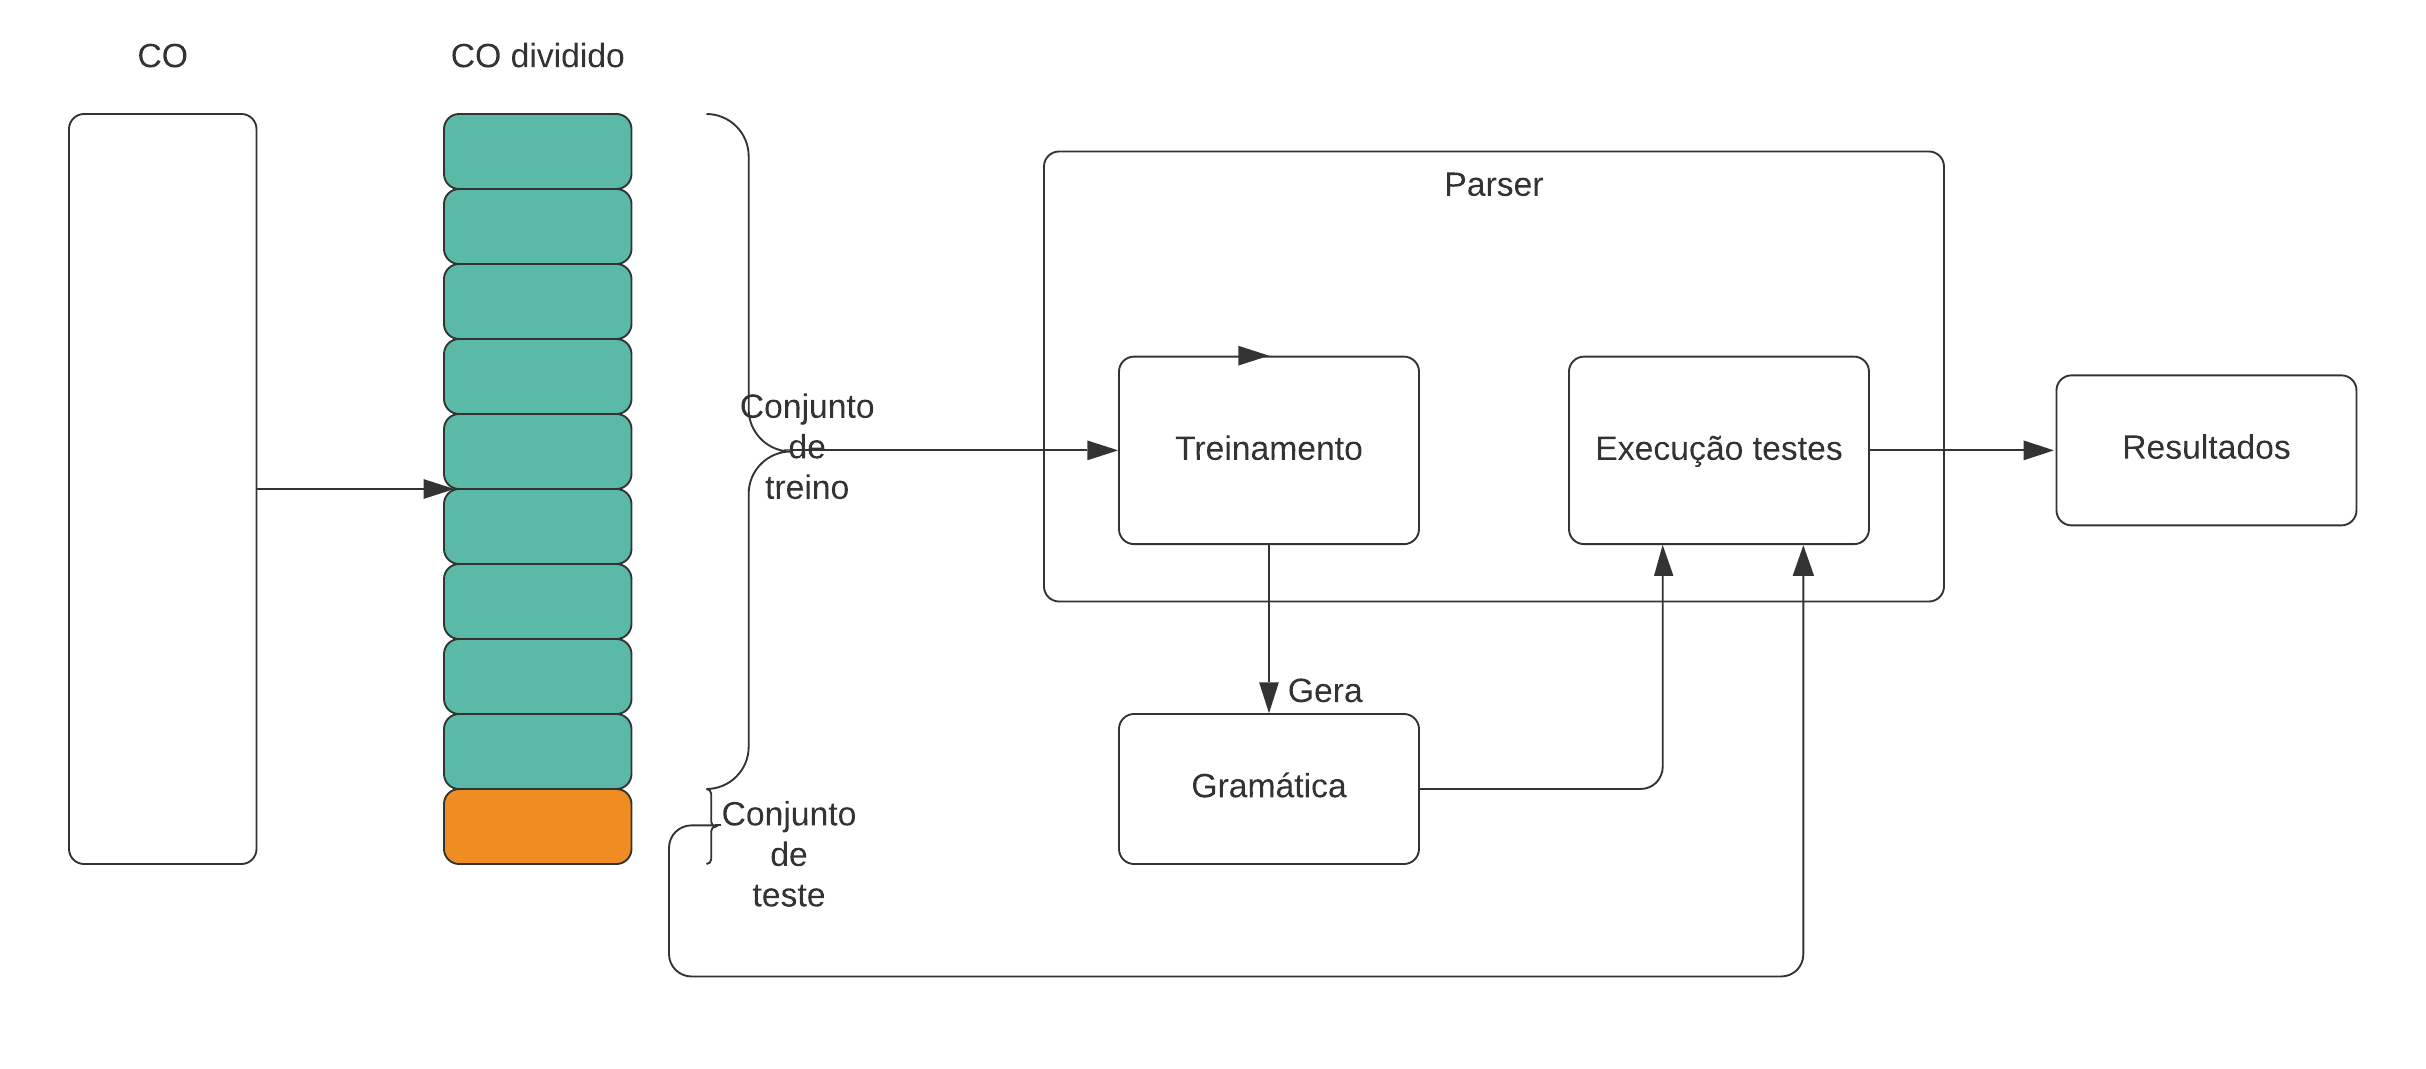
\includegraphics[width=\textwidth,scale=1.5]{imagens/fluxograma_10fold.png}
    \caption[Fluxograma \textit{10-fold validation}]{Fluxograma \textit{10-fold validation}}
    \label{fig:fluxograma_10fold}
\end{figure}
\end{center}

Na sequência, foi executado o treinamento com as partes restantes. De maneira análoga, no mesmo diretório (ou seja, fazendo testes sobre o CINTIL transduzido), foi utilizado o comando \ref{lst:testeBasicoCintil}:

\begin{center}
    \begin{lstlisting}[breaklines, caption={Execução de testes do Stanford Parser para o CINTIL},label={lst:testeBasicoCintil},language=Bash]
    java -cp stanford-parser.jar -mx4g edu.stanford.nlp.parser.lexparser.LexicalizedParser -loadFromSerializedFile /home/fernando/projeto-final-parsers/serialized-files/serialGrammarCINTIL1 input/sentencas_teste_cintil.txt

\end{lstlisting}
\end{center}

Que também merece explicações, na Tabela \ref{tab:tab_teste_basico_cintil}:
\begin{center}
    \begin{table}[h!]
    \centering
    \begin{tabular}{p{0.8\textwidth}}
        \begin{itemize}
            \item [-cp] \textit{ClassPath}. Indica o diretório onde se encontra a classe principal a ser executada
            \item [-mx4g] Quantidade de memória usada. No caso, 4 GB.
            \item [LexicalizedParser] \textit{Parser} utilizado, dentre os disponibilizados
            \item [-writeOutputFiles ] Indica que os testes imprimirão arquivos de saída, a serem definidos
            \item [-outputFilesDirectory] Define o diretório onde os arquivos de saída serão escritos. 
            \item [-loadFromSerializedFile] Carrega a gramática serializada, gerada na execução de treinamento anterior
            \item [-testTreebank] Diretório onde se encontra o treebank a ser usado para teste. Os números no formato $a-b$ indicam o primeiro e o último arquivo, respectivamente. Números no formato $a-b,c-d$ indicam dois blocos de arquivos. Atente para não usar o mesmo bloco dos treinos, ou o parser passará por \textit{overfitting}, e terá resultados enviesados.
        \end{itemize}
    \end{tabular}
    \caption[Comandos para um teste simples do Stanford Parser]{Comandos para um teste simples do Stanford Parser, utilizando o terminal.}
    \label{tab:tab_teste_basico_cintil}
\end{table}
\end{center}

Os treinamentos foram feitos alternando a parte de teste e as partes de treino, totalizando a criação de dez gramáticas, e dez resultados de treinos distintos.

O resultado total dos testes resultou na extensa Tabela \ref{tab:cintil_result_full}, que pode ser vista nos apêndices. E os comentários dos resultados pode ser encontrado em \ref{subsec:resultados_cintil}.

De modo análogo ao CINTIL, fizemos o treinamento baseado num comando simples, como visto no código \ref{lst:treinoBasicoBosque}
\begin{center}
    \begin{lstlisting}[breaklines, caption={Execução de treinos do Stanford Parser para o Bosque},label={lst:treinoBasicoBosque},language=Bash]
    java -cp stanford-parser.jar -mx4g edu.stanford.nlp.parser.lexparser.LexicalizedParser -train ~/<diretorio do treebank> 1-421 -saveToSerializedFile ~/<diretorio de armazenamento>/serialGrammarBOSQUE1 > ~<diretorio de armazenamento>/outputs/treinoBOSQUE/treinoBr1.txt
\end{lstlisting}

\end{center}

São comandos análogos aos supracitados. Explicações podem ser vistas na Tabela \ref{tab:tab_treino_basico_cintil}.

Para a execução dos testes, foi utilizado o comando \ref{lst:testeBasicoBosque}
\begin{center}
    \begin{lstlisting}[breaklines, caption={Execução de testes do Stanford Parser para o Bosque},label={lst:testeBasicoBosque},language=Bash]
    java -cp stanford-parser.jar -mx4g edu.stanford.nlp.parser.lexparser.LexicalizedParser -writeOutputFiles -outputFilesDirectory ~/<diretorio de relatorios de treino>/treino -loadFromSerializedFile ~/<diretorio da gramatica serializada>/serialGrammarBOSQUE1 -testTreebank ~/<diretorio dos treebanks> 422-4213 > ~/<diretorio dos resultados dos testes>testeBr1.txt
\end{lstlisting}

\end{center}

É o mesmo comando explicado na Tabela \ref{tab:tab_teste_basico_cintil}. Também foi utilizado o \textit{10-fold validation} para o Bosque. Porém, os testes foram feitos majoritariamente com o CETEMFolha, que possui 4213 sentenças (contra 10140 do CINTIL).

O resultado completo dos testes pode ser visto na Tabela \ref{tab:bosque_result_full}, nos apêndices. Os comentários dos resultados pode ser visto em \ref{subsec:resultados_bosque}.

Os resultados serão apresentados na Sessão \ref{sec:resultados}.